\section{问题四：调头路径的分段建模与状态递推}
\subsection{问题分解}
问题四给出盘入螺距为1.7 m，要求在半径4.5 m的调头空间内构造盘入与盘出之间的连接路径，并输出$-100$到$100$ s的运动状态。本问先由螺线与调头圆的交点确定调头入点，再按两段相切圆弧和半径比$2:1$建立调头路径，最后在该复合路径上递推全队把手状态。

\subsection{调头曲线的几何关系}
设盘入螺线与盘出螺线关于调头空间中心对称，中间连接段由两段相切圆弧组成，且满足
\[
R_1=2R_2.
\]
为便于表达，设盘入螺线与圆弧1的切点为$P_{\mathrm{in}}$，两圆弧切点为$Q$，圆弧2与盘出螺线切点为$P_{\mathrm{out}}$。那么整条路径由四段拼接而成：
\[
\text{盘入螺线}\to \text{圆弧1}\to \text{圆弧2}\to \text{盘出螺线}.
\]

为了使曲线连续且光滑，相邻段在连接点处应满足位置连续与切向连续。记盘入段与盘出段在边界处的切向单位向量分别为$\bm t_{\mathrm{in}}$和$\bm t_{\mathrm{out}}$，则圆弧1、圆弧2的圆心分别落在对应切点的法线方向上；再结合两圆弧相切与半径比约束，可确定圆心、半径和圆弧转角。

\subsection{固定交点下的几何关系证明}
设盘入螺距为$p=1.7$ m，令
\[
b=\frac{p}{2\pi},\qquad r=b\theta.
\]
调头空间为圆域
\[
\Omega=\{(x,y):x^2+y^2\le R^2\},\qquad R=4.5\ \text{m}.
\]
盘入螺线第一次到达调头圆边界时满足
\[
r(\theta_F)=R,
\]
由此得到入点对应的极角
\[
\theta_F=\frac{R}{b}=\frac{2\pi R}{p}.
\]
对应的交点为
\[
F=P_{\mathrm{in}}=
\bigl(R\cos\theta_F,\ R\sin\theta_F\bigr).
\]
盘出螺线与盘入螺线关于调头空间中心成中心对称，因此出点为
\[
P_{\mathrm{out}}=-P_{\mathrm{in}}.
\]
固定交点情形下的调头曲线几何关系示意图如下。

\begin{figure}[H]
\centering
\placeholderimage{6.2cm}{
图位预留：固定交点调头曲线几何示意图。\\[0.4em]
图中标出调头圆$x^2+y^2=R^2$、盘入螺线$r=b\theta$、盘出螺线的中心对称曲线、\\
交点$F=P_{\mathrm{in}}$、对称点$P_{\mathrm{out}}$、切向量$\bm t_{\mathrm{in}},\bm t_{\mathrm{out}}$、\\
两段相切圆弧的圆心$C_1,C_2$以及圆弧连接点$Q$。
}
\caption{固定交点情形下调头路径的几何关系示意}
\label{fig:q4-fixed-intersection}
\end{figure}

由螺线参数方程
\[
P(\theta)=b\theta(\cos\theta,\sin\theta)
\]
可得切向量
\[
P'(\theta)=b(\cos\theta-\theta\sin\theta,\ \sin\theta+\theta\cos\theta).
\]
于是盘入端点的单位切向量为
\[
\bm t_{\mathrm{in}}=
\frac{P'(\theta_F)}{\|P'(\theta_F)\|}.
\]
记径向单位向量为
\[
\bm e_r=(\cos\theta_F,\sin\theta_F).
\]
设螺线切线与调头圆切线之间的夹角为$\alpha$，则
\[
\alpha=\frac{\pi}{2}-\arccos(\bm t_{\mathrm{in}}\cdot\bm e_r).
\]
将$\bm t_{\mathrm{in}}$代入上式，可得
\[
\alpha
=\frac{\pi}{2}
-\arccos
\frac{(\cos\theta_F-\theta_F\sin\theta_F)\cos\theta_F
+(\sin\theta_F+\theta_F\cos\theta_F)\sin\theta_F}
{\sqrt{\theta_F^2+1}}
=\frac{\pi}{2}-\arccos\frac{1}{\sqrt{\theta_F^2+1}}.
\]
两段圆弧与盘入、盘出螺线相切，且两段圆弧在连接点$Q$处相切。由图\ref{fig:q4-fixed-intersection}中的直角三角关系，圆心连线对应的有效半径和为
\[
R_1+R_2=\frac{R}{\cos\alpha}.
\]
又由题设
\[
R_1=2R_2,
\]
解得
\[
R_1=\frac{2R}{3\cos\alpha},\qquad
R_2=\frac{R}{3\cos\alpha}.
\]
连接点$Q$两侧的圆弧转角相同，均为
\[
\beta=\pi-2\alpha.
\]
于是调头曲线长度为
\[
L_{\mathrm{turn}}
=R_1\beta+R_2\beta
=(R_1+R_2)(\pi-2\alpha)
=\frac{R}{\cos\alpha}(\pi-2\alpha).
\]
其中
\[
\theta_F=\frac{2\pi R}{p},\qquad
\alpha=\frac{\pi}{2}-\arccos\frac{1}{\sqrt{\theta_F^2+1}}.
\]
代入$p=1.7$ m、$R=4.5$ m，得到
\[
\theta_F=16.631961,\quad
\alpha=0.060053,
\]
\[
R_1=3.005418\ \text{m},\quad
R_2=1.502709\ \text{m},
\]
\[
L_{\mathrm{turn}}=13.621245\ \text{m}.
\]

\subsection{路径参数与求解流程}
根据上述几何关系，调头路径满足
\[
\begin{cases}
\text{圆弧1与盘入螺线相切},\\
\text{圆弧1与圆弧2相切},\\
\text{圆弧2与盘出螺线相切},\\
R_1=2R_2,\\
P_{\mathrm{out}}=-P_{\mathrm{in}},\\
P_{\mathrm{in}}=(R\cos\theta_F,R\sin\theta_F).
\end{cases}
\]
求解时先计算$\theta_F$和$\alpha$，再由半径比求$R_1,R_2$，最后按盘入螺线、圆弧1、圆弧2、盘出螺线的顺序建立弧长参数函数。

\begin{algorithm}[H]
\caption{问题四固定交点调头路径与状态求解流程}
\label{alg:q4-turn}
\textbf{Input:} 螺距$p=1.7$，调头空间半径$R=4.5$，整数时刻$t\in[-100,100]$。\\
\textbf{Output:} 调头路径参数、各时刻把手位置与速度。
\begin{enumerate}[label=\arabic*:, leftmargin=2.6em, itemsep=0.2em]
\item 计算盘入螺线与调头圆交点对应的极角$\theta_F=2\pi R/p$。
\item 由交点处螺线切向确定边界切线夹角$\alpha$。
\item 根据$R_1=2R/(3\cos\alpha)$和$R_2=R/(3\cos\alpha)$确定两段圆弧半径。
\item 按盘入螺线、圆弧1、圆弧2、中心对称盘出螺线的顺序建立复合弧长参数路径。
\item 对$t\in[-100,100]$逐秒递推全部把手位置，并由差分计算速度。
\item \textbf{return} 调头路径参数和全队运动状态。
\end{enumerate}
\end{algorithm}

按上述参数得到的调头路径整体示意图如下，用于展示盘入螺线、两段圆弧和盘出螺线的空间拼接关系。

\begin{figure}[H]
\centering
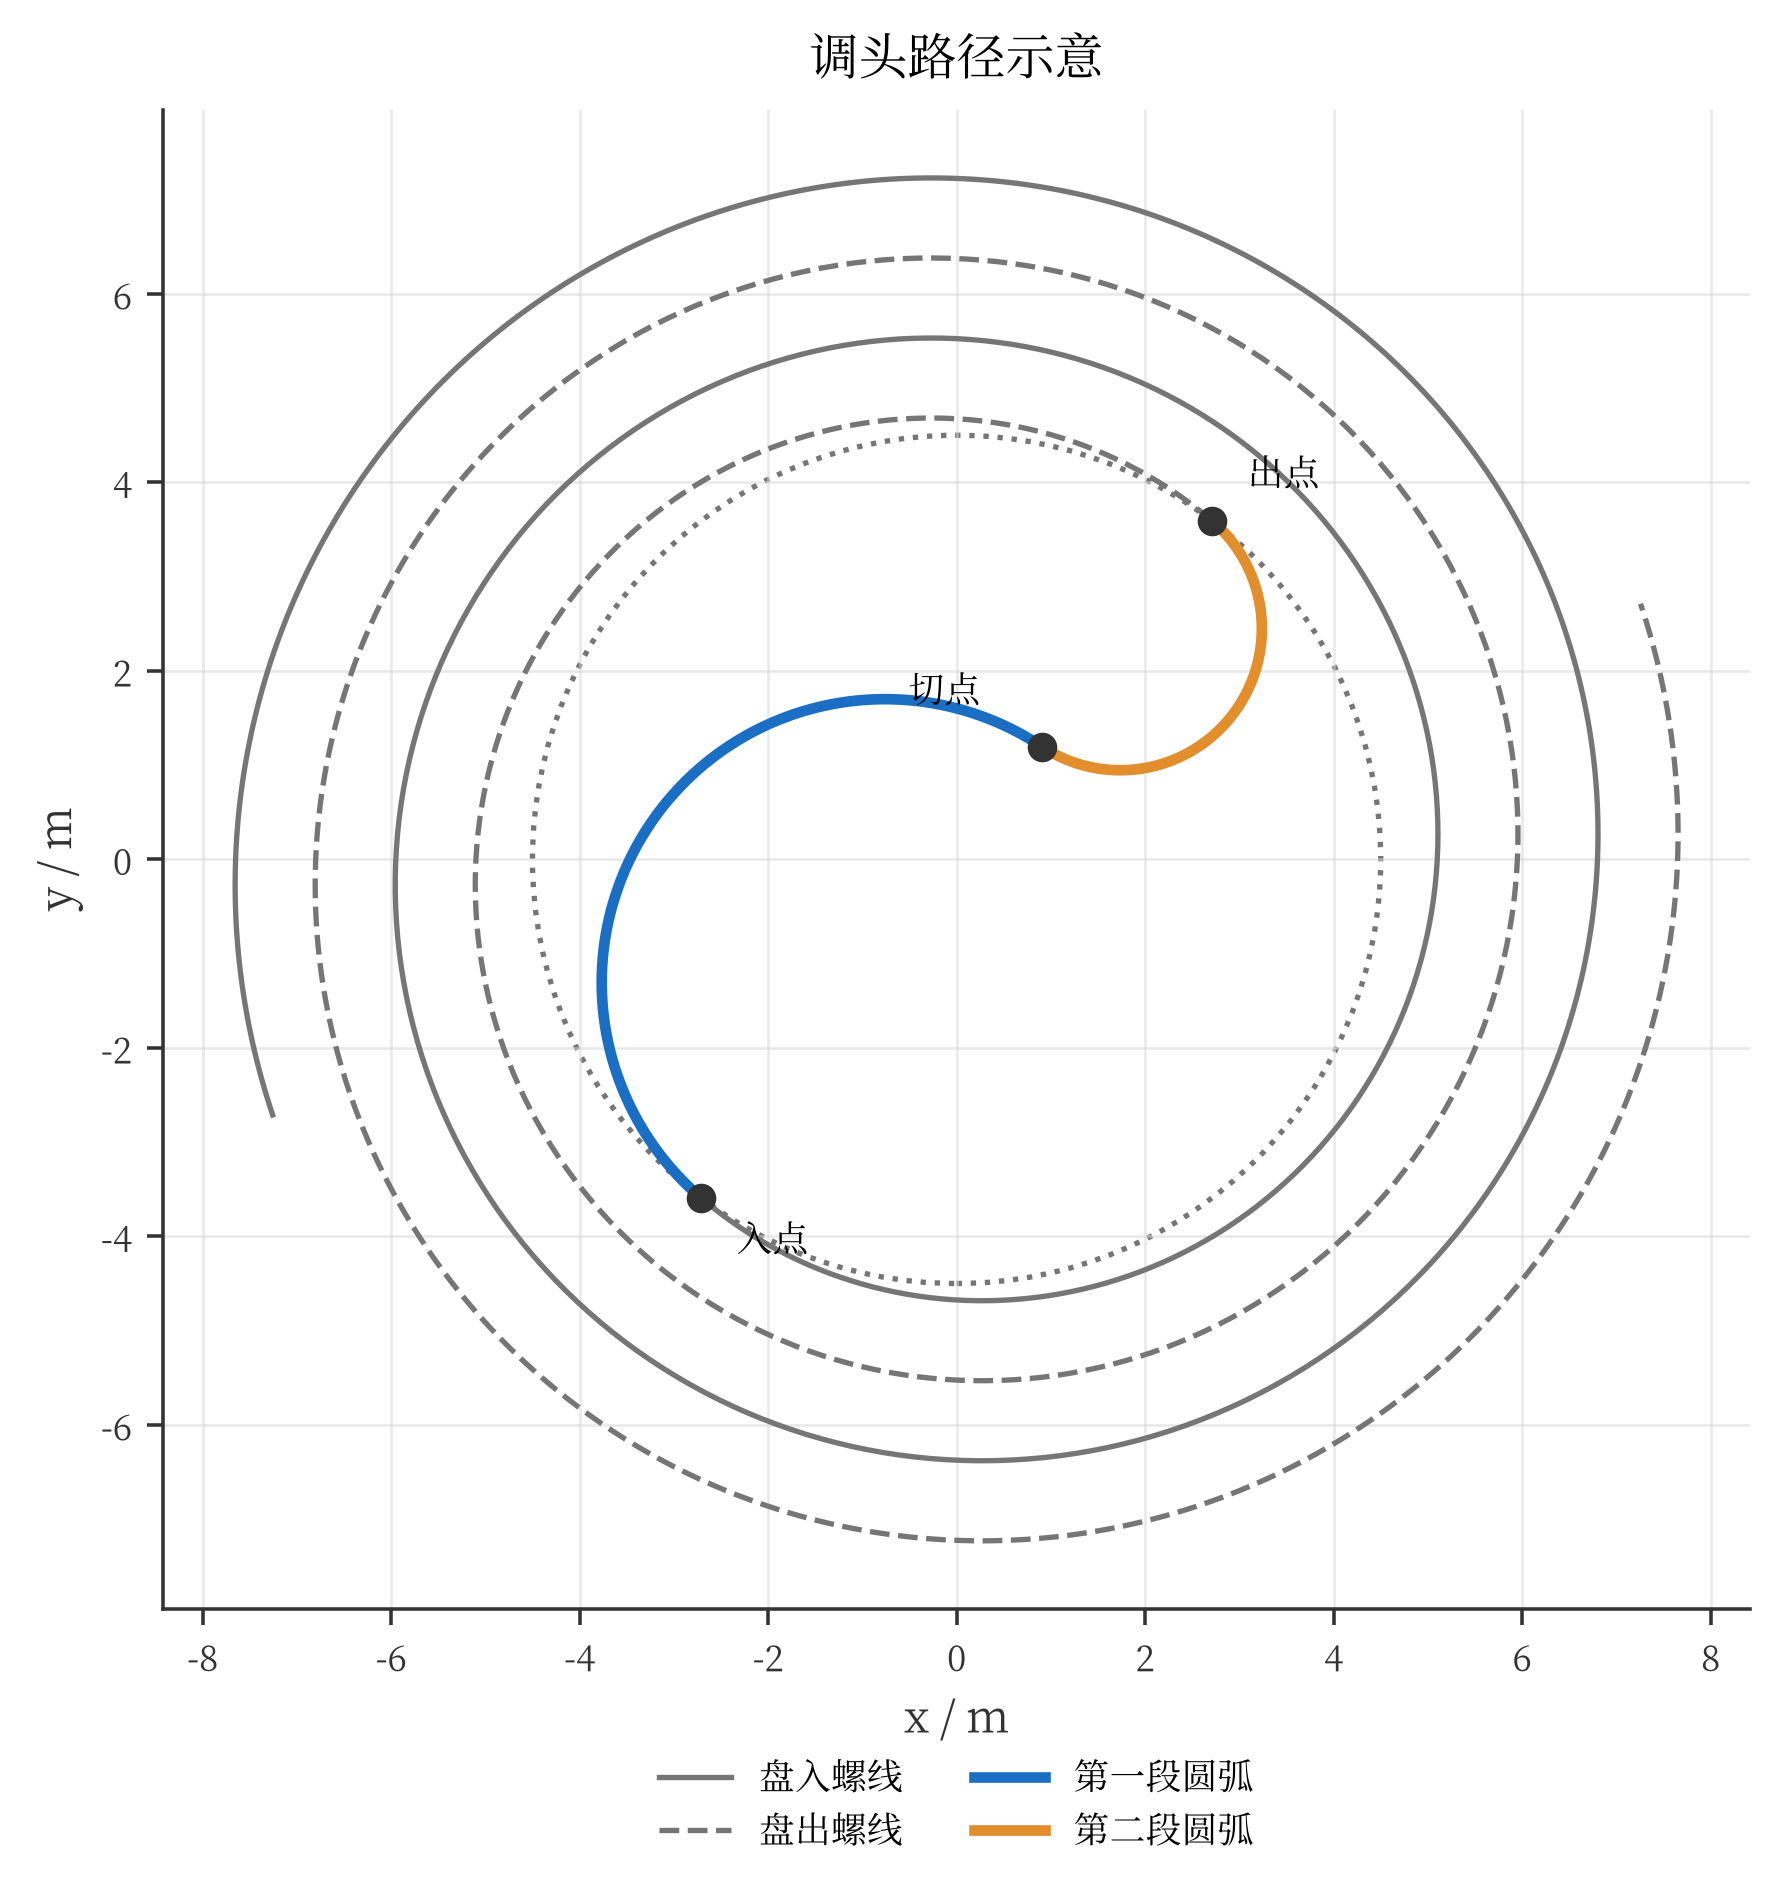
\includegraphics[width=0.92\textwidth]{figures/python/q4_turn_path_overview.png}
\caption{盘入、两段圆弧与盘出路径的整体示意}
\label{fig:q4-turn-path}
\end{figure}

\subsection{状态递推与结果}
在路径确定后，龙头前把手沿该复合路径以1 m/s运动。后续把手仍由固定把手间距逐节递推得到。对于任意时刻$t$，将路径视为弧长参数$s$的函数$P(s)$，先由头速确定龙头对应弧长，再由
\[
\|P_{i+1}(s)-P_i(s)\|_2=d_i
\]
逐节向后求解即可。速度采用问题一中的中心差分形式从位置序列计算。

调头路径参数如下：
\[
R_1=3.005418\ \text{m},\qquad
R_2=1.502709\ \text{m},
\]
\[
L_{\mathrm{turn}}=13.621245\ \text{m}.
\]
整段$-100$到$100$ s的运动状态按上述复合路径递推得到。完整位置表含224个把手在201个整数时刻的$x,y$坐标，规模为$449\times202$；完整速度表含224个把手在201个整数时刻的速度，规模为$225\times202$。两张表已写入结果工作簿\texttt{result4.xlsx}，表\ref{tab:q4-position-extract}和表\ref{tab:q4-speed-extract}列出关键把手在部分时刻的抽样结果。

板凳龙在盘入盘出复合路径上的整体状态示意图如下，用于展示路径改变后全队把手仍按固定距离逐节递推。

\begin{figure}[H]
\centering
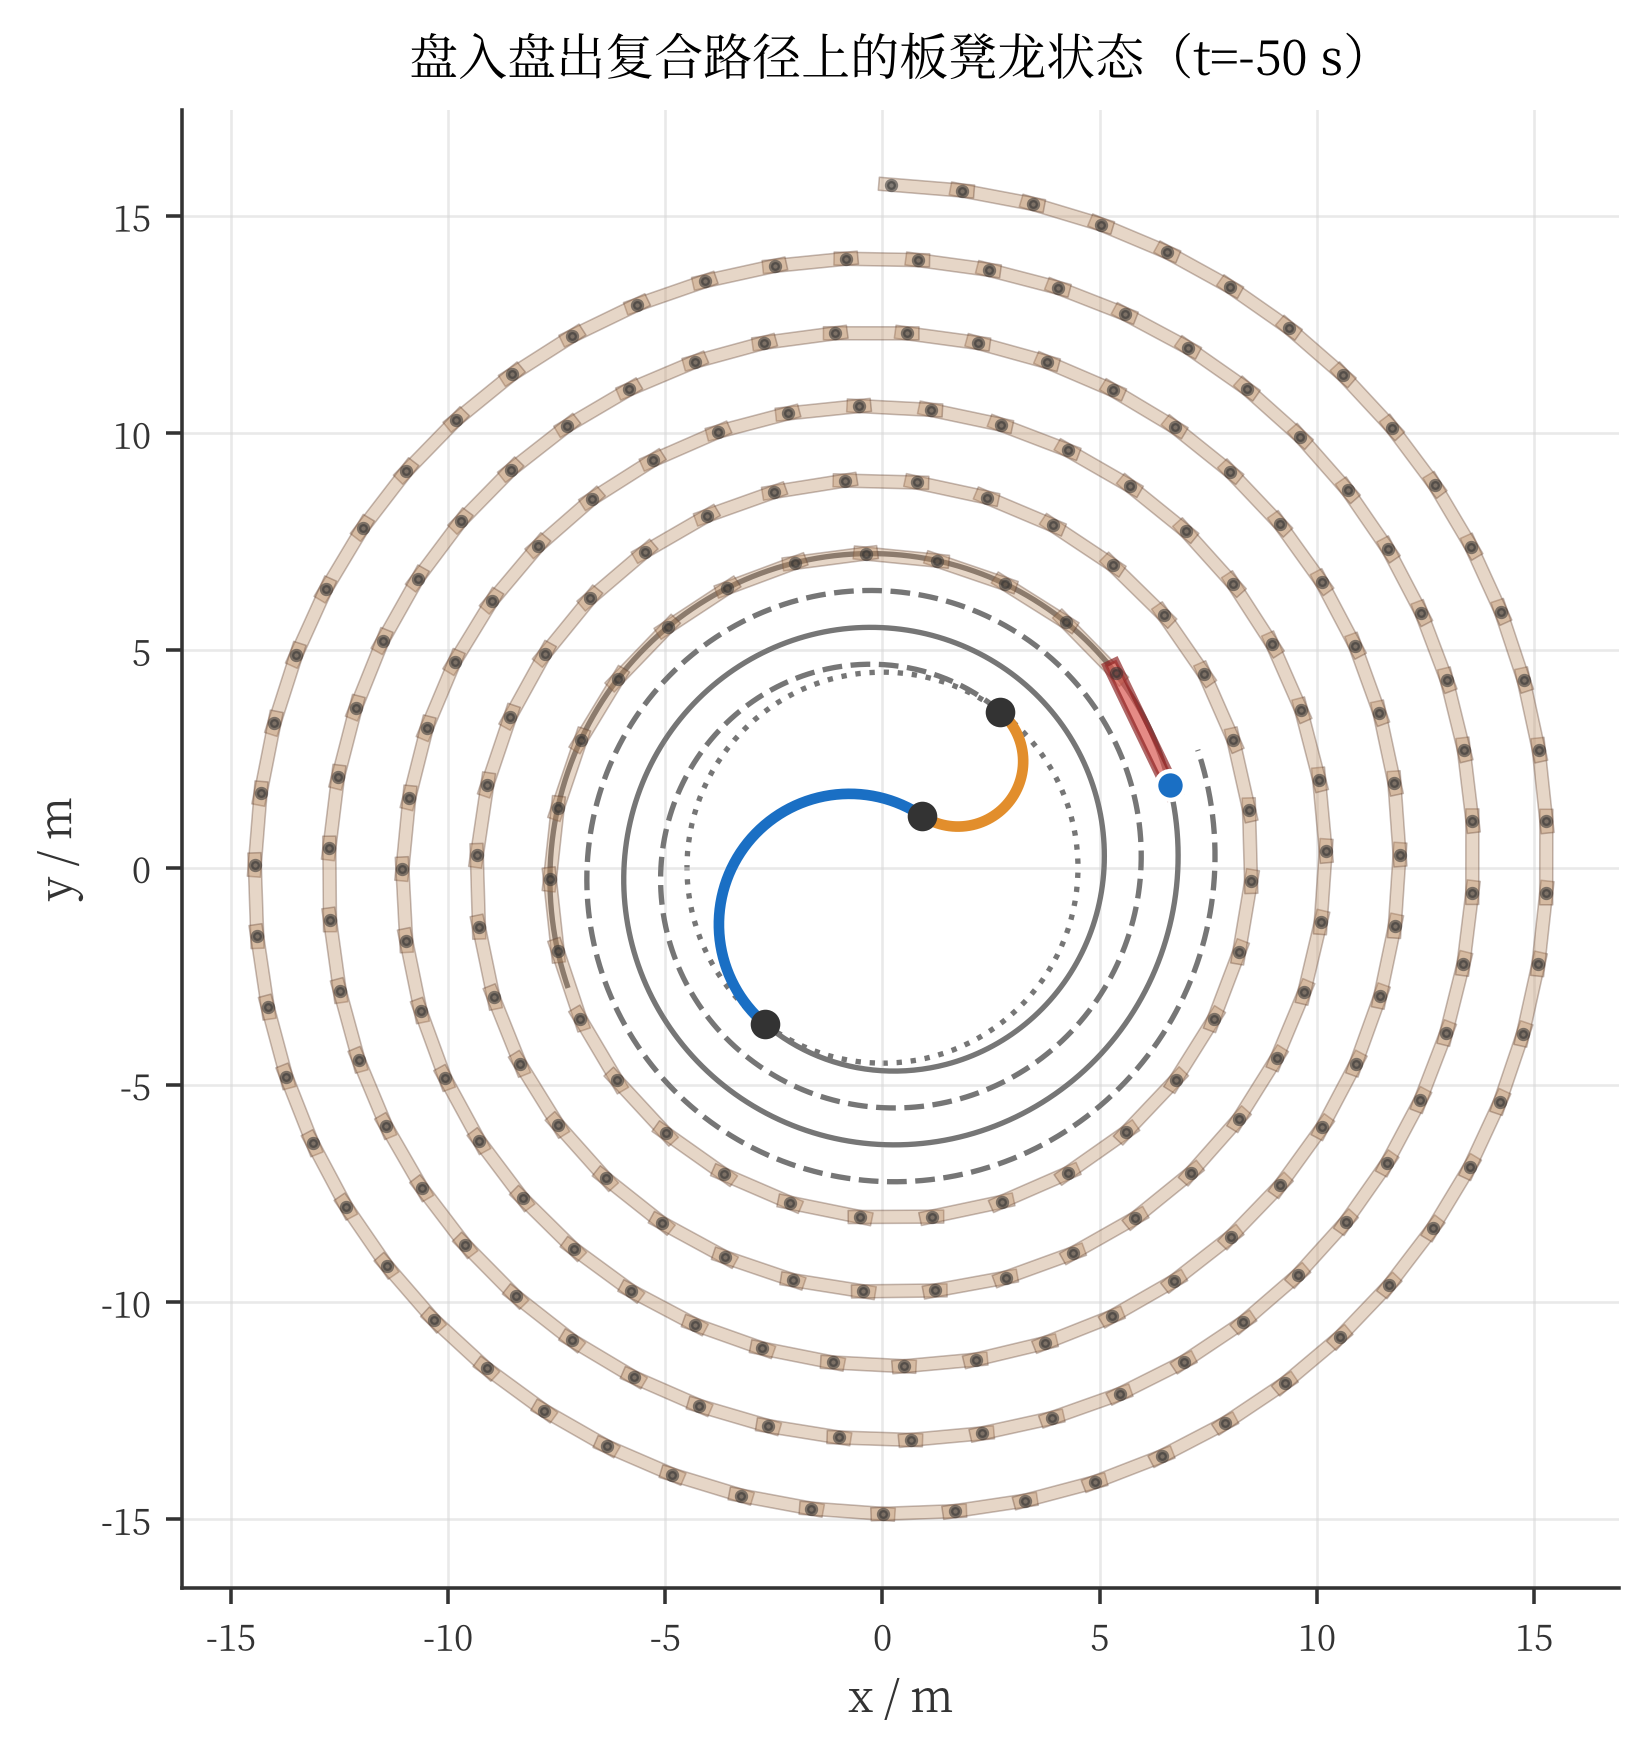
\includegraphics[width=0.92\textwidth]{figures/python/q4_composite_path_state.png}
\caption{板凳龙在盘入盘出复合路径上的状态示意}
\label{fig:q4-inout-snapshot}
\end{figure}

当龙头位于圆弧调头段时的板凳龙状态示意图如下，该图用于说明调头过程中仍采用同一套相邻把手距离递推约束。

\begin{figure}[H]
\centering
\placeholderimage{5.8cm}{
图位预留：板凳龙正在调头时的状态示意图。\\[0.4em]
图中突出显示龙头位于两段圆弧之一时的全队位置，\\
并标注圆弧段、盘入段、盘出段与调头空间边界。
}
\caption{板凳龙处于圆弧调头段时的状态示意}
\label{fig:q4-turning-snapshot}
\end{figure}

\begin{table}[H]
\centering
\caption{问题四调头路径参数表}
\label{tab:q4-result}
\begin{tabularx}{0.86\textwidth}{LCC}
\toprule
量 & 数值 & 单位\\
\midrule
入点极角$\theta_F$ & 16.631961 & rad\\
切线夹角$\alpha$ & 0.060053 & rad\\
圆弧1半径$R_1$ & 3.005418 & m\\
圆弧2半径$R_2$ & 1.502709 & m\\
圆弧转角$\beta$ & 3.021487 & rad\\
调头路径长度$L_{\mathrm{turn}}$ & 13.621245 & m\\
\bottomrule
\end{tabularx}
\end{table}

\begin{table}[H]
\centering
\caption{问题四关键把手位置抽样表}
\label{tab:q4-position-extract}
\begingroup
\setlength{\tabcolsep}{3pt}
\begin{tabularx}{\textwidth}{>{\raggedright\arraybackslash}p{0.15\textwidth}*{5}{R}}
\toprule
项目 & $-100$ s & $-50$ s & $0$ s & $50$ s & $100$ s\\
\midrule
龙头$x$ & 7.778034 & 6.608301 & -2.711856 & 1.332696 & -3.157229\\
龙头$y$ & 3.717164 & 1.898865 & -3.591078 & 6.175324 & 7.548511\\
第1节$x$ & 6.209273 & 5.366911 & -0.063534 & 3.862265 & -0.346890\\
第1节$y$ & 6.108521 & 4.475403 & -4.670888 & 4.840828 & 8.079166\\
第51节$x$ & -10.608038 & -3.629945 & 2.459962 & -1.671385 & 2.095033\\
第51节$y$ & 2.831491 & -8.963800 & -7.778145 & -6.076713 & 4.033787\\
第101节$x$ & -11.922761 & 10.125787 & 3.008493 & -7.591816 & -7.288774\\
第101节$y$ & -4.802378 & -5.972247 & 10.108539 & 5.175487 & 2.063875\\
第151节$x$ & -14.351032 & 12.974784 & -7.002789 & -4.605165 & 9.462513\\
第151节$y$ & -1.980993 & -3.810357 & 10.337482 & -10.386988 & -3.540357\\
第201节$x$ & -11.952942 & 10.522509 & -6.872842 & 0.336952 & 8.524374\\
第201节$y$ & 10.566998 & -10.807425 & 12.382609 & -13.177610 & 8.606933\\
龙尾$x$ & -1.011059 & 0.189809 & -1.933627 & 5.859094 & -10.980157\\
龙尾$y$ & -16.527573 & 15.720588 & -14.713128 & 12.612894 & -6.770006\\
\bottomrule
\end{tabularx}
\endgroup
\end{table}

\begin{table}[H]
\centering
\caption{问题四关键把手速度抽样表}
\label{tab:q4-speed-extract}
\begingroup
\setlength{\tabcolsep}{3pt}
\begin{tabularx}{\textwidth}{>{\raggedright\arraybackslash}p{0.18\textwidth}*{5}{R}}
\toprule
项目 & $-100$ s & $-50$ s & $0$ s & $50$ s & $100$ s\\
\midrule
龙头 & 1.000000 & 1.000000 & 1.000000 & 1.000000 & 1.000000\\
第1节龙身 & 0.999904 & 0.999762 & 0.998687 & 1.000363 & 1.000124\\
第51节龙身 & 0.999346 & 0.998642 & 0.995134 & 0.949935 & 1.003966\\
第101节龙身 & 0.999091 & 0.998248 & 0.994448 & 0.948482 & 1.096263\\
第151节龙身 & 0.998944 & 0.998047 & 0.994156 & 0.948038 & 1.095306\\
第201节龙身 & 0.998849 & 0.997925 & 0.993994 & 0.947823 & 1.094933\\
龙尾（后） & 0.998817 & 0.997885 & 0.993944 & 0.947760 & 1.094833\\
\bottomrule
\end{tabularx}
\endgroup
\end{table}

\subsection{小结}
Q4的核心是在固定交点、两段相切圆弧和半径比$2:1$的约束下建立复合路径，再以该路径为基础计算前后运动状态。该路径下相邻把手距离最大误差为$1.33\times10^{-9}$ m，说明逐节递推在调头前后仍保持了板凳连接约束。
